\documentclass[times, 10pt]{thesisMDH}
\usepackage[ddmmyyyy]{datetime}
\usepackage[pdfborder={0 0 0},colorlinks=true,urlcolor=blue,citecolor=red,bookmarks=false]{hyperref}
\usepackage{float}
\usepackage{makecell}
% \usepackage{indentfirst}
\setlength\parindent{0pt}

\university{University of Science and Technology of Hanoi}
\department{Information and Communication Technology}

\subject{Distributed System}
\thesisTitle{Practical Work 4:\\Word Count}

\authorOne{Nguyen Phuong Thao}{BI9-212}
\authorTwo{Doan Tuyet Mai}{BI9-162}
\authorThree{Trinh Thao Phuong}{BI9-191}
\authorFour{Phung Kim Son}{BI9-202}
\authorFive{Pham Minh Long}{BI9-146}

\theDate{Hanoi, Mar 2021} 

\begin{document}
\titlePage

\newpage

\mainmatter

\section{Why you chose your specific MapReduce implementation?}
We choose to implement by Python because it supports dictionary datatype which is extremely convenient in implementing the Map Reduce. By keeping each word and its occurrence by a key:values pair, we can track which word was counted and combined the occurrence list obtained from Mapper in the Reducer easily.

\section{How your Mapper and Reducer work?}
\begin{figure}[H]
    \centering
    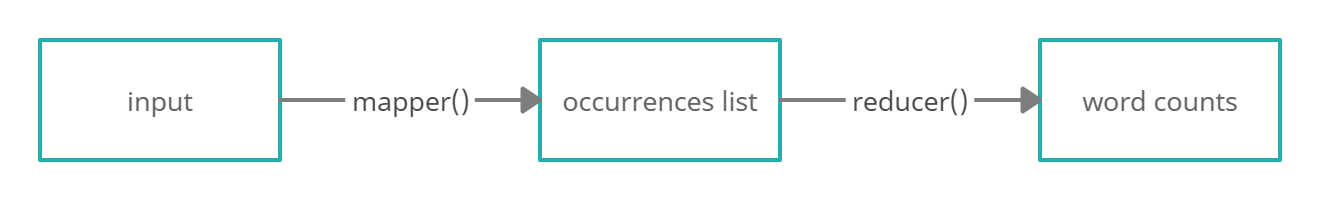
\includegraphics[width=1\linewidth]{images/4-1.png}
    \caption{Mapper and Reducer}
    \label{fig:my_label}
\end{figure}
\subsection{Mapper}
After received the input texts, we run the \verb|strip()| function to remove the leading and trailing whitespace. We also remove the punctuation by doing some \verb|sub("[^\w\s]", "", stc)| method. After that, we split the sentences into words.
\begin{lstlisting}
def mapper(file_name):
	f = open(file_name, "r")
	occurence = []

	for line in f:
		sentences = line.split(".")
		for stc in sentences:
			# Remove leading and trailing whitespace
			stc = stc.strip()

			# Remove punctuation
			stc = re.sub("[^\w\s]", "", stc)

			# Split the line into words
			words = stc.split()

			for word in words:
				#print("%s\t%s" % (word, 1))
				occurence.append([word, 1])

	return occurence
\end{lstlisting}
\subsection{Reducer}
After get the words which are the results of the mapper process, we count the number of each words.
\begin{lstlisting}
def reducer(occurence):
	combined_occ = {}
	for i in range(len(occurence)):
		word = occurence[i][0]
		if word not in combined_occ.keys():
			combined_occ.update({word: 1})
		else:
			occ = combined_occ[word]
			combined_occ.update({word: occ+1})
	return combined_occ
\end{lstlisting}
\section{Contribution}
\begin{center}
    \begin{tabular}{|l|l|l|}
        \hline
        \textbf{Student} & \textbf{Student ID} & \textbf{Contribution}\\
        \hline
        Pham Minh Long & BI9-146 & Write report\\
        \hline
        Phung Kim Son & BI9-202 & Research for different MapReduce implementation\\
        \hline
        Trinh Thao Phuong & BI9-191 & Draw figures, briefly description \\
        \hline
        Doan Tuyet Mai & BI9-162 & Implement code for Word Count (MapReduce) \\
        \hline
        Nguyen Phuong Thao & BI9-212 & Explanation of map reduce\\
        \hline
    \end{tabular}
\end{center}

\end{document}
